\section{Reducción de dimensiones}

\subsection{Introducción}

Disponemos de un dataset de Bag of Words (BOW) que representan descripciones de texto correspondientes a compañías Brasileras clasificadas en nueve categorías distintas. Cada BOW contiene 856 atributos correspondientes a frecuencias de palabras y, debido a la alta dimensionalidad, se busca reducir el conjunto de datos a 3 dimensiones mediante las reglas de aprendizaje de Oja y Sanger.

Regla Oja:
\begin{itemize}
	\item$\Delta W_{ij} = \eta (x_i - \widetilde{x_i}) y_j$
	\item$\widetilde{x_i} = \sum_{j=1}^m y_j . W_{ij}$, donde $m$ es la cantidad de outputs.
\end{itemize}

Regla Sanger:
\begin{itemize}
	\item$\Delta W_{ij} = \eta (x_i - \widetilde{x_i}) y_j$
	\item$\widetilde{x_i} = \sum_{k=1}^j y_k . W_{ik}$
\end{itemize}

\subsection{Modelo}

Cada entrada del dataset contiene 856 atributos, por lo tanto tenemos 856 unidades de entrada. Como queremos reducir el conjuntos de datos a 3 dimensiones, tenemos 3 unidades de salida.

\begin{itemize}
	\item$X \in \mathbb{R}^{856}$
	\item$Y \in \mathbb{R}^3$
	\item$W, \Delta W \in \mathbb{R}^{856\times 3}$
\end{itemize}

\begin{figure}[ht!]
	\centering
	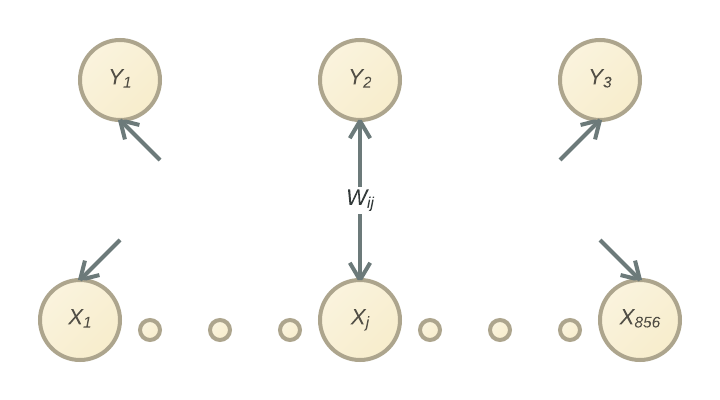
\includegraphics[width=0.7\linewidth]{img/parte1-modelo.png}

	\caption{Modelo de red}
\end{figure}

\subsection{Implementación}

\subsubsection{Prepocesamiento de datos}

El dataset se preprocesa centrando los datos en el 0, calculando la media de las frecuencias de cada palabra (posición del vector) y restándosela a cada una de ellas. De esta forma, la media de cada columna del dataset resultante es 0 y los datos quedan distribuidos alrededor del 0.

\subsubsection{Pseudocódigo}

Inicializamos la matriz de pesos con valores random $\in[-1/2, 1/2]$.

\begin{algorithm}[H]
\caption{train}
\begin{algorithmic}
	\State e = 0
    \While {not fin}
        \State e+=1
        \State lr = lrcons * e$^{-1}$
        \For {x in dataset}
            \State y = x $\bullet$ weights
            \State aplicamos regla
            \State weights += dw
        \EndFor
    \EndWhile
    \State return weights
\end{algorithmic}
\end{algorithm}

\begin{algorithm}[H]
\caption{fin}
\begin{algorithmic}
	\State return (e == max\_epochs) or (weights es ortogonal)
\end{algorithmic}
\end{algorithm}

\begin{algorithm}[H]
\caption{ortogonal}
\begin{algorithmic}
	\State return (weigths$^t$ $\bullet$ weights) - identity matrix $<$ epsilon * identity matrix
\end{algorithmic}
\end{algorithm}


\subsection{Ejecución}

\subsubsection{Modo de uso}

\subsubsection{Requerimientos}

Python

Numpy, Matplotlib